\input{preamble.tex}
\newcommand{\C}{\mathcal{C}}
\pgfplotsset{tick style={very thin}} 


\begin{document}
\pagestyle{fancy}
\fancyhead[L]{Seconde}
\fancyhead[C]{\textbf{Evaluation flash n°3a}}
\fancyhead[R]{\today}

\reversemarginpar

\null\vspace{-30pt}
Nom / Prénom : \\

Consignes particulières : 
\begin{itemize}[label=$\bullet$]
	\item 
	La calculatrice est \textbf{interdite}.
%	\item 
%	Le devoir peut être fait entièrement sur cette feuille.
%	\item 
%	Toute trace de recherche est prise en compte.
	%\item 
	%L'abbréviation $\tq$ signifie ``tel que''.
\end{itemize}

\hrule

\exe{4}{
On donne $f(x) = \dfrac34 x - 3$. 
\begin{enumerate}
\item Donner les paramètres $a$ et $b$ de la fonction affine $f$. 
\item Représenter $\C_f$ dans un repère orthonormé.
\item Le point $P \left ( \dfrac43 ; -2 \right )$ appartient-il à $\C_f$ ? Justifier.
\item Donner l'expression algébrique d'une fonction $g$ telle que les droites $\C_g$ et $\C_f$ soient parallèles et telle que
le point $Q \left ( 1 ; -1 \right )$ appartienne à $\C_g$.
\end{enumerate}
}{exe:1a}{
\begin{enumerate}
\item $a=\dfrac34$ et $b=$-3
\item 
	\begin{center}
	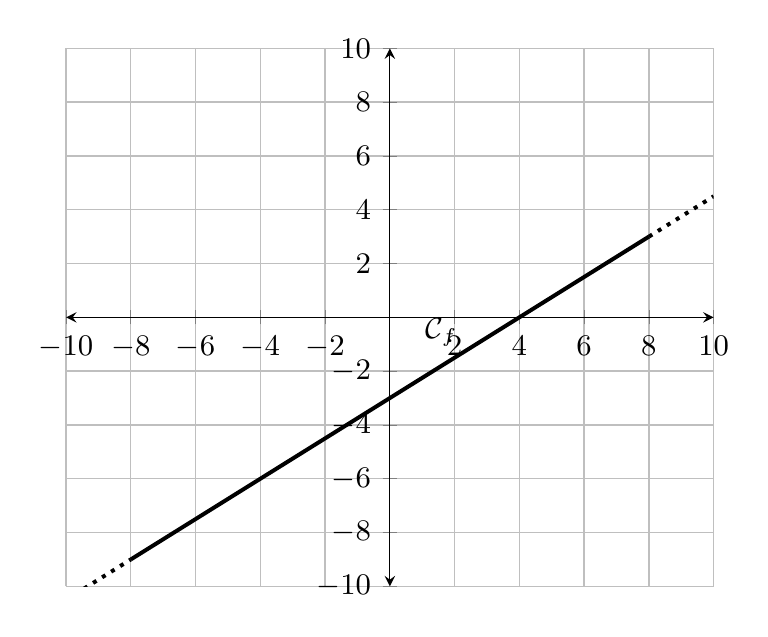
\begin{tikzpicture}[>=stealth, scale=1.2, every node/.append style={font=\small}]
	\begin{axis}[xmin = -10, xmax=10, ymin=-10, ymax=10, axis x line=middle, axis y line=middle, axis line style=<->, xlabel={}, ylabel={}, xtick = {-10, -8, ..., 8, 10}, ytick = {-10, -8, ..., 8, 10}, grid=both]
	
		\addplot[black, very thick, domain =-8:8, samples=2] {3*x/4-3}  node[pos=.6, above=2pt] {$\mathcal{C}_f$};
		\addplot[black, very thick, dotted, domain =-10:-8, samples=2] {3*x/4-3} ;
		\addplot[black, very thick, dotted, domain =8:10, samples=2] {3*x/4-3} ;
	
	\end{axis}
	\end{tikzpicture}
	\end{center}
\item On teste $f  \left ( \dfrac42 \right ) = \dfrac34 \times \dfrac43 - 3 = 1 - 3 = -2$ donc oui.
\item La condition de parallélisme donne le coefficient directeur, donc $g(x) = \dfrac34x + b$.
Pour déterminer $b$ on résout $g(1) = -1$ soit $\dfrac34 + b = -1$ ce qui donne $b=-\dfrac74$.
\end{enumerate}
}

\exe{6}{
On considère les deux droites $\C_f$ et $\C_g$ représentées dans le repère ci-dessous.
	\begin{center}
	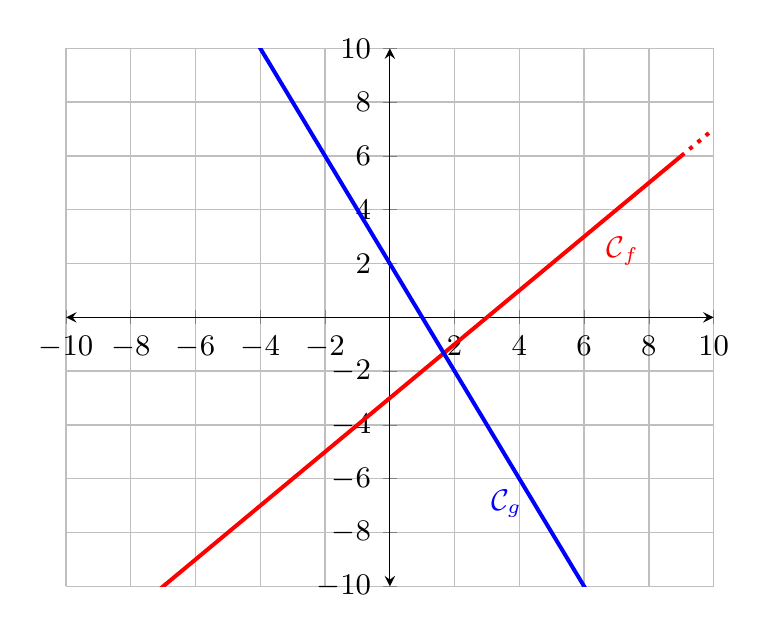
\begin{tikzpicture}[>=stealth, scale=1.2, every node/.append style={font=\small}]
	\begin{axis}[xmin = -10, xmax=10, ymin=-10, ymax=10, axis x line=middle, axis y line=middle, axis line style=<->, xlabel={}, ylabel={}, xtick = {-10, -8, ..., 8, 10}, ytick = {-10, -8, ..., 8, 10}, grid=both]
	
		\addplot[red, very thick, domain =-9:9, samples=2] {x-3}  node[pos=.9, below=6pt] {$\mathcal{C}_f$};
		\addplot[red, very thick, dotted, domain =-10:-9, samples=2] {x-3} ;
		\addplot[red, very thick, dotted, domain =9:10, samples=2] {x-3};
	
	
		\addplot[blue, very thick, domain =-9:9, samples=2] {-2*x+2}  node[pos=.7, below=6pt] {$\mathcal{C}_g$};
		\addplot[blue, very thick, dotted, domain =-10:-9, samples=2] {-2*x+2} ;
		\addplot[blue, very thick, dotted, domain =9:10, samples=2] {-2*x+2};
	\end{axis}
	\end{tikzpicture}
	\end{center}
\begin{enumerate}
\item Pour chacune des droites ci-dessus, donner $2$ points lui appartenant, dont un d'abscisse nulle.
\item Donner les deux ordonnées à l'origine $b$ des fonctions affines associées.
\item Lire graphiquement ou calculer les vecteurs directeurs des deux droites.
\item En déduire les coefficients directeurs $a$ des fonctions affines associées.
\item Ecrire l'expression algébrique des fonctions.
\item Résourdre l'équation $f(x)=g(x)$, en déduire l'abscisse du point $I$ à l'intersection des courbes $\C_f$ et $\C_g$.
\end{enumerate}
}{exe:2a}{
\begin{enumerate}
\item Pour $\C_f$ on a $A(0;-3)$ et $B(3;0)$. \\
Pour $\C_g$ on a $C(0;2)$ et $B(2;-2)$. \\
\item Respectivement $b=-3$ pour $f$ et $b=2$ pour $g$.
\item Pour $f$ : $\vec{AB}=\pvec{3}{3}$ et pour $g$ : $\vec{CD}=\pvec{2}{-4}$
\item On cherche un vecteur colinéaire à $\vec{AB}$ dont la première composante est 1,
soit $\pvec{3}{3}$ colinéaire à $\pvec{1}{1}$ et donc $a=1$ pour $f$. 
En procédant de même, on trouve $a=-2$ pour $g$.
\item $f(x) = x-3$ et $g(x)=-2x+2$.
\item $x-3=-2x+2 \iff 3x=5 \iff x=\dfrac53$.
\end{enumerate}
}

\newpage

\setcounter{Exercise}{0}

\pagestyle{fancy}
\fancyhead[L]{Seconde}
\fancyhead[C]{\textbf{Evaluation flash n°3b}}
\fancyhead[R]{\today}

\reversemarginpar

\null\vspace{-30pt}
Nom / Prénom : \\

Consignes particulières : 
\begin{itemize}[label=$\bullet$]
	\item 
	La calculatrice est \textbf{interdite}.
%	\item 
%	Le devoir peut être fait entièrement sur cette feuille.
%	\item 
%	Toute trace de recherche est prise en compte.
	%\item 
	%L'abbréviation $\tq$ signifie ``tel que''.
\end{itemize}

\hrule

\exe{}{
On donne $f(x) = \dfrac43 x - 2$. 
\begin{enumerate}
\item Donner les paramètres $a$ et $b$ de la fonction affine $f$. 
\item Représenter $\C_f$ dans un repère orthonormé.
\item Le point $P \left ( \dfrac34 ; -1 \right )$ appartient-il à $\C_f$ ? Justifier.
\item Donner l'expression algébrique d'une fonction $g$ telle que les droites $\C_g$ et $\C_f$ soient parallèles et telle que
le point $Q \left ( 1 ; -1 \right )$ appartienne à $\C_g$.
\end{enumerate}
}{exe:1b}{
\begin{enumerate}
\item $a=\dfrac43$ et $b=-2$.
\item 
	\begin{center}
	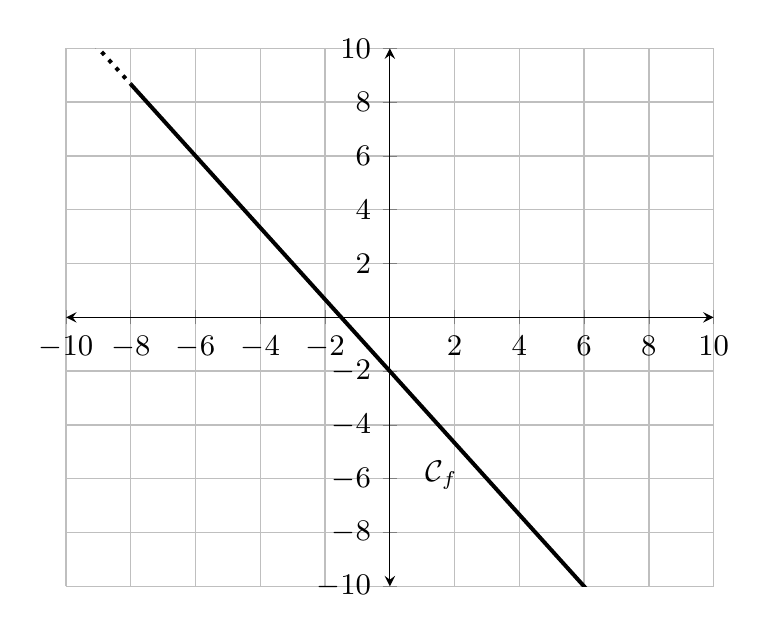
\begin{tikzpicture}[>=stealth, scale=1.2, every node/.append style={font=\small}]
	\begin{axis}[xmin = -10, xmax=10, ymin=-10, ymax=10, axis x line=middle, axis y line=middle, axis line style=<->, xlabel={}, ylabel={}, xtick = {-10, -8, ..., 8, 10}, ytick = {-10, -8, ..., 8, 10}, grid=both]
	
		\addplot[black, very thick, domain =-8:8, samples=2] {-4*x/3-2}  node[pos=.6, below=6pt] {$\mathcal{C}_f$};
		\addplot[black, very thick, dotted, domain =-10:-8, samples=2] {-4*x/3-2} ;
		\addplot[black, very thick, dotted, domain =8:10, samples=2] {-4*x/3-2} ;
	
	\end{axis}
	\end{tikzpicture}
	\end{center}
\item On teste $f  \left ( \dfrac34 \right ) = \dfrac43 \times \dfrac34 - 2 = 1 - 2 = -1$ donc oui.
\item La condition de parallélisme donne le coefficient directeur, donc $g(x) = \dfrac43x + b$.
Pour déterminer $b$ on résout $g(1) = -1$ soit $\dfrac43 + b = -1$ ce qui donne $b=-\dfrac73$.
\end{enumerate}
}

\exe{}{
On considère les deux droites $\C_f$ et $\C_g$ représentées dans le repère ci-dessous.
	\begin{center}
	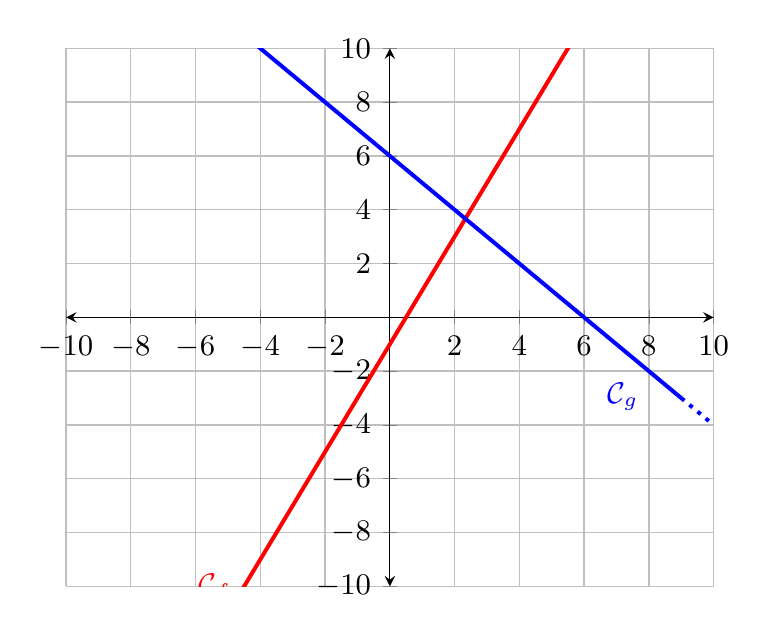
\begin{tikzpicture}[>=stealth, scale=1.2, every node/.append style={font=\small}]
	\begin{axis}[xmin = -10, xmax=10, ymin=-10, ymax=10, axis x line=middle, axis y line=middle, axis line style=<->, xlabel={}, ylabel={}, xtick = {-10, -8, ..., 8, 10}, ytick = {-10, -8, ..., 8, 10}, grid=both]
	
		\addplot[red, very thick, domain =-9:9, samples=2] {2*x-1}  node[pos=.2, above=6pt] {$\mathcal{C}_f$};
		\addplot[red, very thick, dotted, domain =-10:-9, samples=2] {2*x-1} ;
		\addplot[red, very thick, dotted, domain =9:10, samples=2] {2*x-1};
	
	
		\addplot[blue, very thick, domain =-9:9, samples=2] {-x+6}  node[pos=.9, below=6pt] {$\mathcal{C}_g$};
		\addplot[blue, very thick, dotted, domain =-10:-9, samples=2] {-x+6} ;
		\addplot[blue, very thick, dotted, domain =9:10, samples=2] {-x+6};
	\end{axis}
	\end{tikzpicture}
	\end{center}
\begin{enumerate}
\item Pour chacune des droites ci-dessus, donner $2$ points lui appartenant, dont un d'abscisse nulle.
\item Donner les deux ordonnées à l'origine $b$ des fonctions affines associées.
\item Lire graphiquement ou calculer les vecteurs directeurs des deux droites.
\item En déduire les coefficients directeurs $a$ des fonctions affines associées.
\item Ecrire l'expression algébrique des fonctions.
\item Résourdre l'équation $f(x)=g(x)$, en déduire l'abscisse du point $I$ à l'intersection des courbes $\C_f$ et $\C_g$.
\end{enumerate}
}{exe:2b}{
\begin{enumerate}
\item Pour $\C_f$ on a $A(0;-1)$ et $B(2;3)$. \\
Pour $\C_g$ on a $C(0;6)$ et $B(6;0)$. \\
\item Respectivement $b=-1$ pour $f$ et $b=6$ pour $g$.
\item Pour $f$ : $\vec{AB}=\pvec{2}{4}$ et pour $g$ : $\vec{CD}=\pvec{6}{-6}$
\item On cherche un vecteur colinéaire à $\vec{AB}$ dont la première composante est 1,
soit $\pvec{2}{4}$ colinéaire à $\pvec{1}{2}$ et donc $a=2$ pour $f$. 
En procédant de même, on trouve $a=-1$ pour $g$.
\item $f(x) = 2x-1$ et $g(x)=-x+6$.
\item $2x-1=-x+6 \iff 3x=7 \iff x=\dfrac73$.
\end{enumerate}

}


%%%%%%%%%%%%
%
\newpage
\fancyhead[C]{\textbf{Solutions}}
\shipoutAnswer

\end{document}
 